
The main novel idea of our automation engine design is to allow it to solely focus on verification
of functional correctness properties making all good assumptions about other aspects,
e.g., isolation, invariants, interrupts, concurrency, {\it etc}, as given, and provide
a separate systematic framework to handle each of the constructions independent from the functional correctness proof.
We achieve this separation via the technique of \emph{certified abstraction layers}.
In this section, we give a detailed overview our abstraction-layer-based
approach and we illustrate our actual automation engine in Chapter \ref{chapter:automation}.

As in any other system verification, we associate every code module (a piece of code,
or normally, a function)
a specification, and prove that the code meets its specification, or more
formally, there is a {\em forward simulation}~\cite{Lynch95} from the module
implementation to its specification. A specification of a module is a logical
abstract representation of the module's behavior with the concrete
implementation details hidden. We expect the verification to be compositional,
i.e, when we reason about other code modules that utilizes existing verified
module $M$ (e.g., it calls a function in $M$), we expect the verification
of the new modules only looks at the specifications of $M$, given the fact
that $M$ is already proven to meet its specification, so that the verification
never needs to look into the actual implementation of $M$. At the moment $M$ is
being verified, you may not know how $M$ will be used later or what properties of
$M$ may be useful for any global properties you may get interested in.
Thus, we insist the specification of $M$ always capture everything
we may want to know about it. We call such specification a {\em deep specification}.
More formally, for any deep specification $s$, any two implementations that satisfy $s$
should have contextually equivalent observable behaviors. 

When we write a specification for a module, we normally hide the
concrete private data representation in the memory, to ensure the client
of the module can only access the data through defined public interfaces
and thus cannot possibly break any invariants imposed on the private
state in the module implementation. However, in the case of deep
specification, in order to capture any potential behaviors in the
specification itself, we also need to introduce an abstract state
in substitute the concrete private data to use it to specify
full functionality of each public interface of the module.

For example, to specify operations on a doubly
linked list stored in memory, we may logically interpret the complex in-memory
data structure as a simple logical list and specify its {\em push} and {\em pop}
operations as a simple list {\em append} and {\em remove} operations. To support
this, the framework needs to provide a systematic way to hide the private memory
state from its client, and replace them with {\em abstract states} to specify
the full functionality of each operation in the interface in terms of the {\em
abstract states}. It also needs to make sure that this transformation is
sound, i.e., any client code using the {\em push} and {\em pop} operations
on a list should have exactly same behaviors when it is reasoned using the
abstract local specifications and using the concrete doubly linked list
implementation.

\ignore{
Furthermore, a complex system like a kernel module is normally
implemented in a combination of the C and assembly language. Thus, the framework
should be able to be instantiated in both languages and provide a way to
certifiably compile the C-based framework into the assembly-based one. The {\em
certified abstraction layers} provide exactly such support.
}


To better illustrate how the certified abstraction layers work,
in this chapter, we use the verification of a console
circular buffer implementation used in our verified device drivers
as a running example. We show the details step by step and introduce
the concept and definitions used in the verification as they appear.
Fig.~\ref{fig:source:cons-buf} shows the implementation of the circular
buffer in C. The buffer is represented as a circular array
(to store the received input characters) with two additional
fields. The field \texttt{rpos} represents the head of the buffer,
i.e., the index of the next character to read, while the field
\texttt{wpos} indicates the index of the array where the next character
should be written to. When both fields collide, i.e., when both
indexes are the same, it means the buffer is empty. This is why we need
to allocate one extra space (line 2) in order to store \textsf{CB\_SIZE}
characters in the buffer, in which case, the \textsf{wpos} would be
``one index less'' than \textsf{rpos}. 
The figure also defines three functions
\textsf{cb\_init}, \textsf{cb\_read}, and \textsf{cb\_write} that operate
on the circular buffer. The function \textsf{cb\_init} clears the buffer
by setting both \textsf{rpos} and \textsf{wpos} to zero. Note that
it actually suffices to set them arbitrary same value. The function
\textsf{cb\_read} reads a character from the buffer and updates the
indexes accordingly, returning a special character \textsf{CB\_EMPTY}
when the buffer is empty (when the indexes have the same values);
while \textsf{cb\_write} writes a character to the buffer, chopping
off the head character if the buffer was full.

To write a deep specification for the circular buffer, we can use a logical
abstract integer list to represent the in-memory circular buffer implementation.
Then the three operations in Fig.~\ref{fig:source:cons-buf} can be
abstractly specified as they are shown in Fig.~\ref{fig:spec:abs-cons-buf}
using the abstract list as its private data. Here, we use the
notations $[\cdot]$ and $\textsf{++}$ to represent a singleton list and list
concatenation, respectively. The specification shown in
Fig.~\ref{fig:spec:abs-cons-buf} is much cleaner and simpler than the actual
implementation which simplifies future reasoning of code modules that use the
data structure.

\begin{figure}
\lstinputlisting [language = C, multicols=2] {src/console.c}
\caption{Console circular buffer implementation}
\label{fig:source:cons-buf}
\end{figure}

\begin{figure}
\[
\begin{array}{cr}
\inferrule{
}{
	\mathsf{cb\_init} (cb) \defeq \mathsf{nil}
} & \text{(cb\_init)} \\ [5ex]

\inferrule{
	c :: tl = cb \\
}{
	\mathsf{cb\_read} (cb) \defeq (tl, c)
} & \text{(cb\_read\_char)} \\ [3ex]

\inferrule{
	\mathsf{nil} = cb 
}{
	\mathsf{cb\_read} (cb) \defeq (cb, CB\_EMPTY)
} & \text{(cb\_read\_empty)} \\ [5ex]

\inferrule{
	\mathsf{length}~cb < CB\_SIZE \\
}{
	\mathsf{cb\_write} (cb, c) \defeq cb \textsf{++} [c]
} & \text{(cb\_write\_char)} \\ [3ex]

\inferrule{
	h :: tl = cb \\
	\mathsf{length}~cb = CB\_SIZE \\
}{
	\mathsf{cb\_write} (cb, c) \defeq tl~\textsf{++}~[c]
} & \text{(cb\_write\_overflow)} \\
\end{array}
\]
\caption{Specifications of abstract console buffer primitives}
\label{fig:spec:abs-cons-buf}
\end{figure}

Next, we show how we can prove the abstract deep specification
is equivalent to the actual C implementation in arbitrary client context.
We first show how we represent the abstract states and primitives
in our framework.
Then we show the source language our code module is implemented in,
how we reason about the source code written in the language utilizing
the abstract states and primitives,
and how we link everything to reach the final
{\em contextual refinement} property we seek for.

In this chapter and the following chapters, I try my best to present the exact
implementations of example definitions, specifications, and proofs
directly in Coq, instead of in an invented logical notations
(like derivation rules in Fig.~\ref{fig:spec:abs-cons-buf}).
The purpose is to help the readers to better understand how the certified
abstraction layers are implemented in Coq in our framework, instead of
merely getting the high level ideas. The hope is to make it easier for others to
reproduce our work for their own purpose.


\section{Layer Interface}
\label{sec:layer_interface}
To support the deep specification, the framework needs a formal notion
that can be used to represent an arbitrary list of abstract states,
and a set of abstract primitives that operate on the abstract states. 
Furthermore, the framework should be able to enforce a set of system
invariants on the abstract states which gets preserved across
the system execution, especially by the abstract primitives.
A {\em layer interface} serves such a purpose.

A layer interface $L$ consists of the {\em abstract states}, {\em
  primitives}, a set of {\em invariants} on the abstract states, and
{\em proofs} that all the primitives in the layer interface preserves
the layer invariants.  An {\em abstract state} could be a logical
state that does not correspond to any physical state in the machine,
but in most cases, it is a logical state that is abstracted from a
concrete state in the registers or memory. Each {\em primitive}
operates (exclusively) on the abstract states and is associated with an atomic
specification. It is abstracted from a concrete, verified piece of the
actual code.  

\begin{figure}
\lstinputlisting [language = Coq] {src/cons_buf_spec.v}
\caption{Specifications of abstract console buffer in Coq}
\label{fig:cons_buf_spec}
\end{figure}

As an example, we show how we implement a layer interface in Coq
for the abstract console buffer shown in Fig.~\ref{fig:source:cons-buf}
and \ref{fig:spec:abs-cons-buf}. Fig.~\ref{fig:cons_buf_spec} shows
our actual Coq implementation. First, the type of abstract states
is always defined as a Coq \textsf{Record} with each record field
representing concrete abstract state.
As explained before, the abstract console buffer (named \textsf{cb})
is represented as a Coq list of integers (line 1-4).
Line 6 to 20 shows the specifications of three abstract primitives
in Coq. Here, $cb~d$ represents retrieving the field $cb$ from the
abstract state $d$, and $d~\{cb: newcb\}$ indicates a new abstract state
$d'$ with the field $cb$ equal to the provided new value $newcb$ and
otherwise the same as $d$. The specifications shown in Fig.~\ref{fig:cons_buf_spec}
are the Coq implementations of the ones presented in Fig.~\ref{fig:spec:abs-cons-buf}.

Furthermore, we also define an invariant over the abstract buffer
in this layer interface.

\begin{invariant}[valid console buffer length]
\begin{align*}
0 \leq \textsf{Zlength} (d.cb) \leq \textsf{CB\_SIZE}
\end{align*}
\end{invariant}

The invariant says that the length of abstract buffer should always
be between zero and the given maximum size.
It is not hard to prove that all of the three primitives preserves
this invariant.

Given the layer interface, we need a way to incorporate the layer interface
into our source language so that the code implemented in the source language
can utilize the primitives to manipulate the abstract states, while always
maintaining the data invariants. Our framework support both a C-like
language ClightX (which is an extension to the CompCert Clight language
with our layer interface) and an x86-based assembly language LAsm
(which is an extension to the CompCert Asm language for the x86
architecture with layer interface). In the subsequent sections,
we first define these two languages formally, then present
a formal notion of {\em certified abstraction layers} that can be used
to verify the code modules with deep specifications.

\ignore{
Since the {\em invariants} are preserved by all the
primitives, the abstract states can only be accessed through calling
one of the primitives, and execution of the primitives are atomic, the
invariants hold at any moment during the system execution.
}


\section{Language ClightX}

\begin{figure}
\lstinputlisting [language = Coq] {src/clight_expr.v}
\caption{Clight expressions}
\label{fig:clight_expr}
\end{figure}

\begin{figure}
\lstinputlisting [language = Coq] {src/clight_stmt.v}
\caption{Clight statements}
\label{fig:clight_stmt}
\end{figure}

In this section, we introduce the language ClightX, which is the C-like
language our framework supports. 
The language ClightX is an extension of the language Clight~\cite{blazy-leroy-clight}
supporting the layer interfaces. We first present the language Clight in detail.

Language Clight is a subset of C and is
formalized in Coq as part of the CompCert project~\cite{compcert}.  Its formal
semantics relies on a memory model~\cite{leroy08} that is not only
realistic enough to specify C pointer operations, but also designed to
simplify reasoning about non-aliasing of different variables.
From the programmer's point of view, 
Clight avoids most pitfalls and peculiarities of C such
as nondeterminism in expressions with side effects. 
On the other hand,
Clight allows for pointer arithmetic and is a true subset of C: valid
Clight programs are valid C programs with the same semantics.
Such simplicity and practicality turn Clight into a solid choice for
certified programming.
Furthermore, the CompCert verified compiler
provides strong guarantees on code
obtained by compilation of Clight programs.

\subsection{Syntax of Clight}

Fig.~\ref{fig:clight_expr} and Fig.~\ref{fig:clight_stmt} shows the formal
definitions of Clight expressions and statements in Coq, respectively.
With the help of comments, the figures should be self-explanatory.

Note that Clight expression is free of side effects. Thus, a function
in Clight cannot be an expression, as executing the function body
may trigger side effects, e.g., it may change the system state like the memory.
Instead, as shown in the figure, a function call is a statement in Clight,
and in order to support the assignment of the form $v = f(a_1, \cdots, a_n)$, the
statement \textsf{Scall} takes an optional variable identifier as the first  argument,
which represents the variable we would like to write the return value to.
It is optional because the function may not have any return value, or the return
value may get discarded instead of getting written to a variable, i.e.,
it maybe simply of the form $f(a_1, \cdots, a_n)$ in the standard C format.

Furthermore, Clight only defines an infinite loop
(line 10 in Fig.~\ref{fig:clight_stmt}), and the common C loop constructors
like \textsf{while}, \textsf{do while}, and \textsf{for} loops are defined
separately in terms of the infinite loop \textsf{Sloop} (line 25-32
in Fig.~\ref{fig:clight_stmt}). 
In our verified code, we never use
the \textsf{goto} statement.
The language also supports special set of functions built into the language.
They are not used in our framework, and thus are omitted from Fig.~\ref{fig:clight_stmt}.

\subsection{Semantics of Clight}

Next, we present the formal semantics of Clight. CompCert defines
both a small-step and a big-step semantics for Clight, which are proven
to be equivalent. In this subsection,
we only present the big-step semantics, as it is simple and our automated
verification tactics is designed based on it.

\paragraph{Clight States}
Clight states consist of following components.
\begin{itemize}[leftmargin=*]

\item Memory state \textsf{m} of type \textsf{mem} is the main memory
that uses the CompCert memory model. Instead of viewing the main memory
as a huge consecutive sequence, the memory is represented as a list of
disjoint CompCert memory blocks. A pointer to the memory is represented
by a block id and an offset within the block (offsets starts from zero).
Each block has its own size and it is not allowed to go beyond the block boundary
or move to another block through any pointer arithmetic operations.
Full details can be found in ~\cite{leroy08}.  

\item Global environment \textsf{ge} of type \textsf{genv} represents the mapping
from global variable/function identifiers to the memory blocks that the variables/functions
are stored. Since CompCert memory stores each global variable and function into
its own memory block, storing the offset is not necessary (it is always zero).
This mapping is fixed once the system code is fixed and can be constructed
before the system executes the main function. Thus, during the execution, 
this mapping never changes.

\item Local variable environment \textsf{e} of type \textsf{env} gives the
mapping from the local variable identifiers to their memory locations
(memory block and offset). Note that since more than one local variables
could be on the same memory block (e.g., on the same stack), the mapping
in this case also gives the block offset. This mapping also does not change
during the system execution since no variable locations vary during the system
execution, though their values stored in those locations may change during the
execution.

\item Local temporary environment \textsf{le} of type \textsf{temp\_env} is
a mapping from local temporary variables to their actual values. Temporary
variables are special variables in Clight designed for optimization and
they are not stored in memory (similar to the register variables in GCC).
When we generate the Clight code, we can scan the code and find
all the variables that are never taken address of, and represent
them using the temporary variables
instead of the above local variables. Given that they are never taken the
address of, it is not necessary to store them in the memory, and we just need
to keep the logical mapping from their identifiers to their actual values.
The compiler optimization can then save them in the registers instead of memory
if possible. Note that since the mapping saves the actual values of the temporaries,
\textsf{le} changes during the system execution.


\end{itemize}


\paragraph{Expression Evaluation}
Fig.~\ref{fig:clight_eval_expr} shows the rules for evaluating Clight
expressions. The definition is parameterized over the memory $m$,
global environment $ge$, variable environment $e$, and the temporary
environment $le$. Note that Clight expressions do not produce any
side effects. That means evaluating Clight expressions does not
change any of the above system states.
As shown in Fig.~\ref{fig:clight_eval_expr}, the rules are defined inductively
with each constructor corresponds to some expression shown in Fig.~\ref{fig:clight_expr}.
The inductive definitions for evaluating right and left values are defined
mutually recursively.

\paragraph{Statement Execution}
Fig.~\ref{fig:clight_exec_stmt} and Fig.~\ref{fig:clight_exec_stmt2}
shows the big-step semantics on executing the Clight statements.
The inductively defined predicate \textsf{exec\_stmt} takes
the Clight states and a Clight statement, and produces
an event trace, a new temporary environment and memory, and
an execution outcome. Here, the event trace \textsf{t} of type
\textsf{trace} is used to represent the list
of external observable events. It is not used in our verified system, thus
the value of trace \textsf{t} is always the empty trace \textsf{E0}.
The execution outcome \textsf{out} of type \textsf{outcome} indicates how
the execution terminated, either normally (\textsf{Out\_normal}), or prematurely
through a break (\textsf{Out\_break}) or a continue (\textsf{Out\_continue})
statement. The value \textsf{Out\_return} of type $option~(val * type)$ is used to indicate
the termination by returning a value of given type, or \textsf{None} if
just by returning with no return value.

Fig.~\ref{fig:clight_exec_stmt} shows the semantic constructors for a subset
of Clight statements. The majority of the rules in the figure should be
self-explanatory. Note that there are two rules for the sequential compositions
(line 15-22), where the first rule (line 15-18) represents the case when
both composed statements executes sequentially (the first statement terminates
with \textsf{Out\_normal}), while the second rule (line 19-22) explains
the case when the execution of first rule stops abnormally and the whole sequence
terminates without executing the second statement.

Fig.~\ref{fig:clight_exec_stmt2} presents the semantic rules for more
complex statements, i.e., loops and function calls.
The various predicates related to the execution outcome is defined in
Fig.~\ref{fig:clight_outcomes}.

Recall that Clight defines only one native loop constructor called \textsf{Sloop},
where the common loop definitions are derived from \textsf{Sloop}.
As shown in the figure, there are three execution rules for the loop $\textsf{Sloop}~s1~s2$.
The main rule \textsf{exec\_Sloop\_loop} (line 14-19) represents the case
when both $s1$ and $s2$ terminates normally and the loop gets into the next iteration.
It first executes the first statement $s1$ (line 15) that terminates normally (line 16),
then it runs the second statement $s2$ (line 17), and continues the next iteration (line 17).
Note that the termination due to the \textsf{continue} statement is also
considered normal (line 16), since \textsf{continue} simply means not to execute
the subsequent statements in the loop body, but does not mean to terminate the loop.
The other two rules for the loops are the cases when the loop terminates.
The rule \textsf{exec\_Sloop\_stop1} represents the case when running the first statement
(line 5) terminates abnormally through the \textsf{break} or \textsf{return} statements
(line 6), in which case it terminates the entire loop.
The second rule \textsf{exec\_Sloop\_stop2} shows the case when running the first
statement (line 9) terminates normally (line 10), but the execution of the second
statement (line 11) stops abnormally (line 12), which again causes the entire execution
to jump out of the loop.

There is a single rule for executing a function call statement
$\textsf{Scall}~optid~a~al$.
Understanding this rule is critical in getting the idea on how we extend the
Clight language with the layer interfaces. As shown in
Fig.~\ref{fig:clight_exec_stmt2}, it first checks whether the type
of the function expression is valid, i.e., whether the type of $a$ is
either a function or a function pointer (line 21).
Then the function expression $a$ is evaluated (line 22), followed
by the evaluation of the argument list $al$ (line 23). After some sanity checks
(line 24 and 25), the function is evaluated with the argument values
(line 26) and the result is written to the optional variable in the $optid$
if necessary (the \textsf{set\_opttemp} part in line 27).
The predicate \textsf{eval\_funcall} that actually evaluates the function
is defined mutually recursively below in the figure. 
As shown in the figure, there are two kinds of functions in Clight.
One is the internal function that is implemented within the module,
which is evaluated by executing the function body recursively using
the \textsf{exec\_stmt} predicate above (line 32), and the other
is called external functions used to represent the functions from
some external sources that get linked with the current module.
Clight requires every external function to provide the semantics on
how the call changes the system states, which is encapsulated in
the \textsf{external\_call} predicate (line 35). It also requires
the proof that the semantics satisfies a list of predefined properties
to respect the compiler correctness.

\begin{figure}
\lstinputlisting [language = Coq] {src/clight_eval_expr.v}
\caption{Evaluation rules for Clight expressions}
\label{fig:clight_eval_expr}
\end{figure}

\begin{figure}
\lstinputlisting [language = Coq] {src/clight_exec_stmt.v}
\caption{Big-step semantics for Clight: part 1}
\label{fig:clight_exec_stmt}
\end{figure}

\begin{figure}
\lstinputlisting [language = Coq] {src/clight_exec_stmt2.v}
\caption{Big-step semantics for Clight: part 2}
\label{fig:clight_exec_stmt2}
\end{figure}

\begin{figure}
\lstinputlisting [language = Coq] {src/clight_outcomes.v}
\caption{Outcomes of statement execution}
\label{fig:clight_outcomes}
\end{figure}


\subsection{Extending Clight to ClightX}

The key idea behind deep specification and the layer-based approach
is to gradually abstract the in-memory private data into simpler logical
abstract states and the functions manipulating the private data
into logical atomic primitives operating on the abstract states instead.
Thus, we need a way to extend Clight so that the language can be instantiated
with different layer interfaces. In other words, the language ClightX
needs to be parametric over a layer interface $L$. 
The standard Clight semantics is unaware of either the
abstract states or the abstract primitives defined in the layer
interface. Therefore, there are two challenges
in this extension. First, the state of Clight language should be extended
to support the abstract states. Second, we also need to support
the abstract primitives so that we can syntactically invoke these primitives
in the ClightX source code and the semantics of these primitive calls
should be able to update the abstract states.

On the other hand, we seek to minimize the impact on the existing proof
infrastructure for program and compiler verification. Thus, we do not
modify the semantics of basic operations of Clight, but access the
abstract states exclusively through the Clight's external function
mechanism provided in Clight. Recall that
Clight axiomatizes the behaviors of external functions without
specifying them, and only assumes they do not behave in a manner that
violates compiler correctness. We use the external function mechanism
to extend Clight with our primitive operations, and supply their
specifications to make the semantics of external functions precise. 
The remaining challenge is that, as shown in the line 37 of
Fig.~\ref{fig:clight_exec_stmt2}, the type of external function semantics
are already fixed by Clight and it does not contain the new abstract states
as mutable states in the type. Fortunately, the memory model used in
the Clight semantics is an axiomatized memory model, which does not
give any concrete implementation, for example, on the concrete type
of the memory. Thus, we instrument original memory type $mem$ as a
new pair $mem * RData$, and instrument the memory access operation
to access the first part of this new pair. This allows us not to change
any of the old Clight semantics for the old operations of Clight,
while still be able to give semantics to the external functions (primitives)
that changes the abstract state part (the second element in the pair)
of the new memory type.

As a result, the language ClightX is parametric over the layer interface,
or more specifically, the type of abstract states $RData$ (as the second
element in the memory pair), and the list of abstract primitives (as the
list of available external functions) specified using the memory pair
(the memory and the abstract states).

The specification of external functions in ClightX (shown in line 37 of
Fig.~\ref{fig:clight_exec_stmt2}) is defined as an inductive predicate,
and operates on both the memory and abstract states (thanks to the parameterization
of the memory as a pair). On the other hand, the semantics of ClightX is
deterministic given a layer interface. Furthermore, in majority of the
cases, the primitive in the layer interface does not change the main memory.
This is because, we always try to first abstract the memory into logical
abstract states and specify the primitives in terms of the abstract
states. Thus, in our framework, the specifications of primitives
are mostly written as a Coq function, as they were shown in Fig.~\ref{fig:cons_buf_spec}.
We have implemented a simple transformer that converts the functional form
into predicates when they are passed to ClightX. The functional form
is more concise and readable. Another benefit is that we do not need to
prove each primitive specification satisfies the external call properties
defined in CompCert. They are proved once and for all in the transformer.

\subsection{Code Module in ClightX}

Given the definition of the language ClightX above,
we can implement the code modules, e.g., the console buffer
implementation shown in Fig.~\ref{fig:source:cons-buf}, in ClightX
and formally reason about their properties using the formal semantics
of ClightX. On the other hand, the ClightX syntax is defined
in the abstract syntax form, which is very inconvenient
to write comparing to the standard C format. Instead,
our ClightX code is automatically generated from standard C code
through a tool called $\textsf{clightgen}$ provided by CompCert~\cite{compcert}.
We directly verify the generated ClightX code. Thus, correctness
of the $\textsf{clightgen}$ does not affect the correctness of
the verified code.

For simplicity, in the examples used throughout the thesis, we show
the source code directly in the standard C, even though in Coq, they
are implemented in ClightX.


\section{Language LAsm}
Even though majority of the system software is implement in C,
we would like our formal claim to be made at the actual compiled assembly
code running on the machine. Furthermore, many of the system software
has some snippet of code directly implemented in assembly.
Thus, we need a formal notion of an assembly language with
the support of parametric layer interface.

\subsection{Syntax and Semantics of LAsm}

The language LAsm is a super set of the CompCert x86 assembly language with more
machine-dependent registers and instructions needed for implementing
low level system software. 
Fig.~\ref{fig:lasm_regs} shows the register definitions in LAsm.
They are mostly consistent with the standard x86 assembly language,
except the special pseudo register $RA$ representing the return
address (line 26). In x86, the return address is normally stored
on the stack when a function is called, but in LAsm (also in
CompCert assembly) it is saved in this special pseudo register $RA$.
It is called a pseudo register because it does not really exist
in a physical machine. 

Fig.~\ref{fig:lasm_instructions} presents a small subset of assembly
instructions in LAsm, with their small-step formal semantics
detailed in Fig.~\ref{fig:lasm_semantics}.
The statements and their semantics are
mostly similar to the standard x86 assembly language, except the
special treatment of stack with the two {\it Pallocframe} and {\it Pfreeframe}
pseudo instructions. In actual x86, the stack is a consecutive sequence
of memory, but CompCert memory model cannot reflect that stack blocks
are adjacent and they are allocated and freed following some stack disciplines.
Instead, CompCert memory model introduces the two pseudo instructions
to allocate and deallocate stack blocks which get pretty-printed later
into appropriate stack increment and decrement x86 instructions. 
As shown in Fig.~\ref{fig:lasm_semantics}, {\it Pallocframe} first allocates
a new memory block of specified size and saves the old stack pointer and return
address into the block at specified offsets, while {\it Pfreeframe} restores
the old stack pointer and return address saved in the block and frees the memory
block.

To support parametric layer interfaces, the semantics of LAsm is also instrumented
in the similar way ClightX is extended from Clight.
As shown in Fig.~\ref{fig:lasm_step}, we have introduced a new kind of
external function \texttt{exec\_step\_prim\_call} for assembly-style primitives
in addition to the external function \texttt{exec\_step\_external} for C-style primitives.
This is necessary because a module directly implemented LAsm may not follow the C
calling convention. Note that the ``style'' here denotes the calling convention,
and not the language the module is implemented in. For example, C-style
primitives can certainly be implemented in LAsm as long as it follows the C calling
convention.


\begin{figure}
\lstinputlisting [language = Coq] {src/asm_regs.v}
\caption{Registers in LAsm}
\label{fig:lasm_regs}
\end{figure}

\begin{figure}
\lstinputlisting [language = Coq] {src/asm_instructions.v}
\caption{Instructions in LAsm}
\label{fig:lasm_instructions}
\end{figure}

\begin{figure}
\lstinputlisting [language = Coq] {src/asm_semantics.v}
\caption{Formal Semantics of LAsm}
\label{fig:lasm_semantics}
\end{figure}

\begin{figure}
\lstinputlisting [language = Coq] {src/asm_step.v}
\caption{Execution Rules of LAsm Instructions}
\label{fig:lasm_step}
\end{figure}


\subsection{Code Module in LAsm}

Unlike the case of ClightX, code modules implemented in LAsm are
directly written manually. This is acceptable because LAsm syntax
is not quite verbose, and especially because the portion of the code
directly implemented in assembly is normally quite small in most
of system software.

The verified ClightX
source code can be compiled by our extended CompCertX compiler
\cite{dscal15} to the corresponding LAsm assembly in such a way that
all proofs at the Clight level are preserved at the LAsm level. Then,
the compiled LAsm modules and their proofs can be linked with the ones
directly developed in LAsm.


\section{Certified Abstraction Layer} 

We have formally defined the source languages and how we parameterize
their semantics with respect to a layer interface. 
This allows us to implement code modules like the circular console
buffer in Fig.~\ref{fig:source:cons-buf}, and specify them
within the layer interface shown in Fig.~\ref{fig:cons_buf_spec}.
Next, intuitively, we would like
to formally express and prove the property that the implementation
of the circular buffer in Fig.~\ref{fig:source:cons-buf} and the specifications
in the layer interface in Fig.~\ref{fig:cons_buf_spec} are {\em equivalent}
in some sense under any program context. 
A {\em certified layer} allows us to achieve that.

\subsection{Certified Layer and Contextual Refinement}

A {\em certified layer} is a new language-based
module that consists of a triple $\layer{L_1}{M}{L_2}$ plus a mechanized proof
object showing that the layer implementation $M$ that is built on top of the
layer interface $L_1$ (the {\em underlay interface}), i.e.,
$\llbracket{}M\rrbracket{}L_1$, is a {\em contextual refinement} of the
desirable layer interface $L_2$ above (the {\em overlay interface}).

\begin{definition}[Contextual Refinement]
We say that $\llbracket{}M\rrbracket{}L_1$ contextually refines
$L_2$ if, and only if, for any module (context) $P$ disjoint from $M$,
the behavior of $\llbracket{}{P \oplus M}\rrbracket{}L_1$ is subset of
that of $\llbracket{}P\rrbracket{}L_2$.
\end{definition}

\begin{figure}
\begin{center}
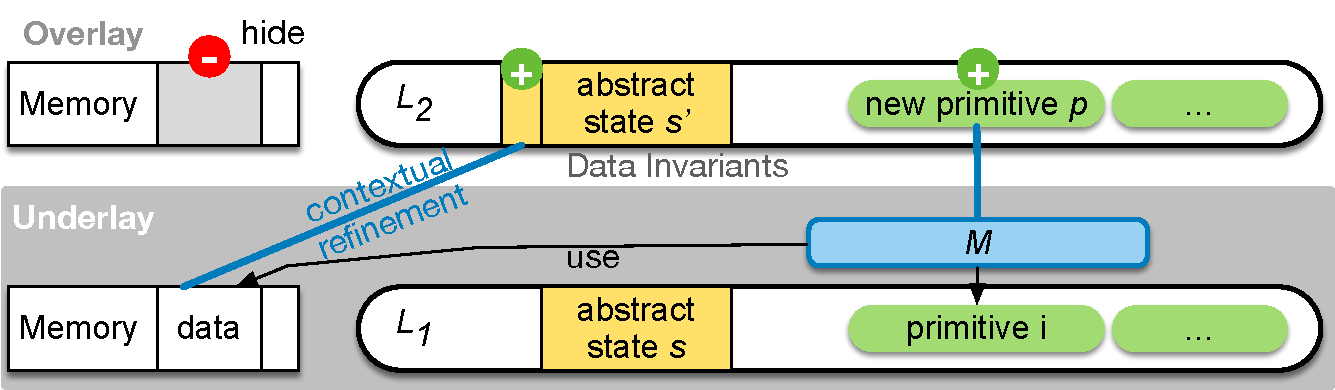
\includegraphics[width=0.8\textwidth]{figs/object-original}
\end{center}
\caption{Layer-based contextual refinement}
\label{fig:spec:object-original}
\end{figure}


Given that $\llbracket{}M\rrbracket{}L_1$ contextually refines $L_2$,
and the deep specifications in $L_2$ captures everything contextually observable
about running $M$ over its underlay $L_1$, we can prove any property of $M$ directly using
the interface $L_2$ alone, and we would never need to look into the actual
implementations in $M$. Since all of our specifications are deterministic
(under fixed external events), the contextual refinement property guarantees
that $\llbracket{}M\rrbracket{}L_1$ and $L_2$ are actually observably equivalent.

Fig.~\ref{fig:spec:object-original} shows the overall idea of the contextual
refinement. As shown in the figure, the code module $M$ may access some
private data in the memory, which corresponds to the new abstract states
in the overlay interface $L_2$. Note that $M$ may also call some of the
primitives defined in the underlay interface $L_1$. The entire behavior
of $M$ is specified as the new abstract primitives in $L_2$ manipulating
the new abstract states in $L_2$ instead. Given that the memory in $L_1$
is replaced by the abstract states in $L_2$, we would like to 
guarantee that the context
code running on the overlay interface does not accidentally damage the private
in-memory data by directly accessing the relevant memory. As shown in
Fig.~\ref{fig:spec:object-original}, we achieve this by utilizing the CompCert
memory permissions~\cite{leroy08} to hide the relevant memory region at overlay,
which prevents the context code from accessing the relevant memory. These
logical permissions do not correspond to any physical protection mechanism, but
are used to ensure that the abstract machine at overlay gets stuck if any code
tries to directly access this portion of memory. The safety proof of our entire
system (the system never gets stuck) guarantees that such a situation never
happens. Thus, the only way to affects the abstracted memory by any context code
running over the overlay interface $L_2$ is to explicitly call relevant
primitives in $L_2$.

\subsection{Downward Simulation}

The contextual refinement is proven by showing a forward
simulation~\cite{Lynch95} between $L_2$
to $\llbracket{}M\rrbracket{}L_1$ over a refinement relation.
In the rest of the chapter, following CompCert, we often call the
forward simulation $\llbracket{}M\rrbracket{}L_1$ (implementation)
to $L_2$ (specification) as {\em upward (forward) simulation} and
the one from $L_2$ (specification) to $\llbracket{}M\rrbracket{}L_1$
(implementation) as {\em downward (forward) simulation}.
The contextual refinement, by definition, requires us to prove
the {\em upward simulation} from $\llbracket{}M\rrbracket{}L_1$
to $L_2$. In practice, the {\em downward simulation} is easier to
achieve, and this is what we prove in our framework. Relying
on the fact that the specifications are deterministic, the proof
is then later turned into the converse {\em upward simulation}
similar to the the way in CompCert.

\begin{definition}[Downward Simulation]
We say that there is a downward simulation from $L_2$ to
$\llbracket{}M\rrbracket{}L_1$ if, and only if, for any
context program $P$ disjoint from $M$, there exists a refinement relation
$R$ over the two states in $\llbracket{}P\rrbracket{}L_2$ and
$\llbracket{}{P \oplus M}\rrbracket{}L_1$ such that, for
every state $(s_2, s_1)$ in $R$, and for every step $st$ in $\llbracket{}P\rrbracket{}L_2$,
if $st$ takes the state from $s_2$ to $s_2'$, then there exists
zero or more steps in $\llbracket{}{P \oplus M}\rrbracket{}L_1$ from
$s_1$ to $s_1'$ such that $(s_2', s_1')$ is also in $R$.
\end{definition}

\subsection{Finding Refinement Relation}

To show the downward simulation, we need to find a simulation relation $R$
such that every step in $\llbracket{}P\rrbracket{}L_2$ can be simulated by
some steps in $\llbracket{}{P \oplus M}\rrbracket{}L_1$.
As shown in Fig.~\ref{fig:spec:object-original}, the relation $R$ can
map the memory and abstract states in $L_2$ to the same memory and abstract
states in $L_1$, with the exception of the part of memory that is hidden in
$L_2$ and the new abstract states introduced in $L_2$. Since the part of
memory is hidden in $L_2$, this part of memory is not mapped to
the same memory containing private data in $L_1$, and in fact it is not
mapped to any state in $L_1$. Instead, the new abstract states in $L_2$
is mapped to the concrete private data in $L_1$'s memory. The concrete
mappings vary depending on the concrete data structures used to implement
the in-memory private data in $L_1$, and the format used to represent
its corresponding abstract states in $L_2$. In the example of the console
buffer, $R$ needs to match the concrete circular array in the memory
to the abstract logical list defined in the layer interface.


\subsection{Proving Downward Simulation}

Based on the definition of the downward simulation, the simulation needs
to be shown for every step in $\llbracket{}P\rrbracket{}L_2$.
Note that the only step that needs special
attention is when $P$ calls one of new primitives introduced in $L_2$.
Because for any other
steps, $\llbracket{}{P \oplus M}\rrbracket{}L_1$ can make exactly same step
to reach a matching state at the underlay.
When $P$ calls any one of the new primitives in $L_2$, this can be simulated
by running the corresponding function defined in $M$ at the underlay.

Thus, in our framework, one only needs to provide the simulation proof
from each overlay primitive $p$ to the corresponding underlay function
implementation $f$, primitive by primitive, with respect to a provided
refinement relation $R$. For each primitive that takes an overlay state
$s_2$ and produces a new state $s_2'$, this proof contains two components.
The first part is to show that from the underlay state $s_1$ that matches to
$s_2$ in $R$, the function $f$ (written either in ClightX or LAsm)
terminates safely and transforms the state $s_1$ to another state $s_1'$.
This step requires us to reason about the function $f$ based on its formal
semantics, and prove that the function does terminate safely (i.e., it
does not get stuck or get into an infinite loop) and produce the return state
$s_1'$. The second part is to show that $s_1'$ is also related to $s_2'$ by $R$.

Instead of mixing these two proof together, our framework provides a way to
systematically isolate these two otherwise related proofs. First, we write
a new specification for each function $f$ in terms of the underlay states.
This specification is called {\em low level specification} in our framework,
in contrast to the {\em high level specification} of the primitive at overlay
in terms of the overlay states. Next, we prove that $f$ satisfies its
{\em low level specification}. This step is called {\em code verification}.
Last, we prove the simulation from the (high level) specification of $p$ to the
{\em low level specification} for $f$ over the refinement relation $R$.
This is called the {\em refinement proof}. The advantage of splitting these
two works are that we do not need to worry about the simulation when we
perform the {\em code verification}, while no code is involved when
we establish the {\em refinement proof}.

A low level specification has a similar type as the primitive
(high level) specification in a layer interface.
As an example, the low level specification for the console buffer
implementation (shown in Fig.~\ref{fig:source:cons-buf}) is shown
in Fig.~\ref{fig:cons_buf_low_spec}.
Here, $\textsf{lspec}~ ge~ args~ (m,~d)~ rval~ (m',~d')$
indicates that under the global environment ($ge$) mapping global variable
identifiers to their locations in the (CompCert) memory, given the argument list
$args$, the function changes the memory from $m$ to $m'$ and the abstract
state from $d$ to $d'$, with the return value
$rval$ ($\textsf{Vundef}$ if no return value). $\textsf{Mem.store}$ is an
operation in the CompCert memory model;  it takes the memory writing type, initial
memory to write to, the memory block, block offset, and a value, and returns the
new memory after writing the value on the location represented by the memory
block and offset on the initial memory. $\textsf{Mem.load}$ is the opposite
operation that loads a value in the specified location of the memory.

\ignore{
As shown in the figure, the low level specifications has equivalent
number of cases as in the source code, and in fact, they are very close
to the source code. Thus, it is relatively easy to show that the source code
satisfies the low level specification shown in
Fig.~\ref{fig:cons_buf_low_spec} and the proof can be achieved nearly
automatically by our proof tactics.
}

\begin{figure}
\lstinputlisting [language = Coq] {src/cons_buf_low_spec.v}
\caption{Low level specifications of the circular console buffer}
\label{fig:cons_buf_low_spec}
\end{figure}


\subsection{Layer Patterns}
As shown in the previous subsection, there are two main components in proving the
downward simulation: the {\it refinement proof} that deals with the relationship
between the overlay abstract states and underlay states, and the {\it code verification}
that handles the verification of actual functional properties of the program.
To further ease the task of developing the layer interfaces and proving the
downward simulation, we have designed and developed two common patterns which
can be used to decompose the problems into pieces so that we only need to focus
on one type of proof at a single moment.

When we introduce and verify a code module, we always first perform {\it data abstraction},
i.e., we abstract the concrete data stored in the underlay memory into a logical
abstract states in the overlay, and provide very simple getter/setter interface in
the overlay to manipulate the new abstract states. The getter and setter methods
are implemented at underlay with simple memory accesses that does not involve much
complex logic or cases. Thus, the {\it code verification} is relatively simple in this case
given the simplicity of the code and similarity between the specification and the
implementation of getters and setters. The main proof focus of this pattern would
be the {\it refinement proof} where we have to show the equivalence of the abstract
and concrete representations of the data. The complexity of this task highly depends
on the complexity of in-memory data structures used and the actual representation
of the abstract states at overlay. It may get very complex when the gap between 
the two representations are relatively large (as in the case of circular console buffer).

Once all the in-memory data are abstracted into logical states at overlay with
the getter/setter interfaces, we implement the actual functional logic on top
of the previous overlay by utilizing the getter/setter primitives whenever
we need to access the new abstract states. Here, the {\it refinement proof}
is trivial as there is no data abstraction, thus the refinement relation is
the {\it identity relation}. The major proof task in this pattern is to perform
the actual {\it code verification}, and we detail our techniques in Chapter
\ref{chapter:automation}.

We have discovered that following the above two patterns significantly reduces the
amount of proof efforts required to prove complex systems by only focusing on one
of the two main proof tasks while completely automating the other.
It also allows us to implement much stronger automation support for each isolated
proof component because, for example, there is no complex code logic involved in the
data abstraction, and the code only manipulates logical states during the
code verification, thus no direct manipulation of the CompCert memory.


\section{Back to Console Circular Buffer}
\label{chapter:framework:console-buffer}

\begin{figure}
	\begin{center}
		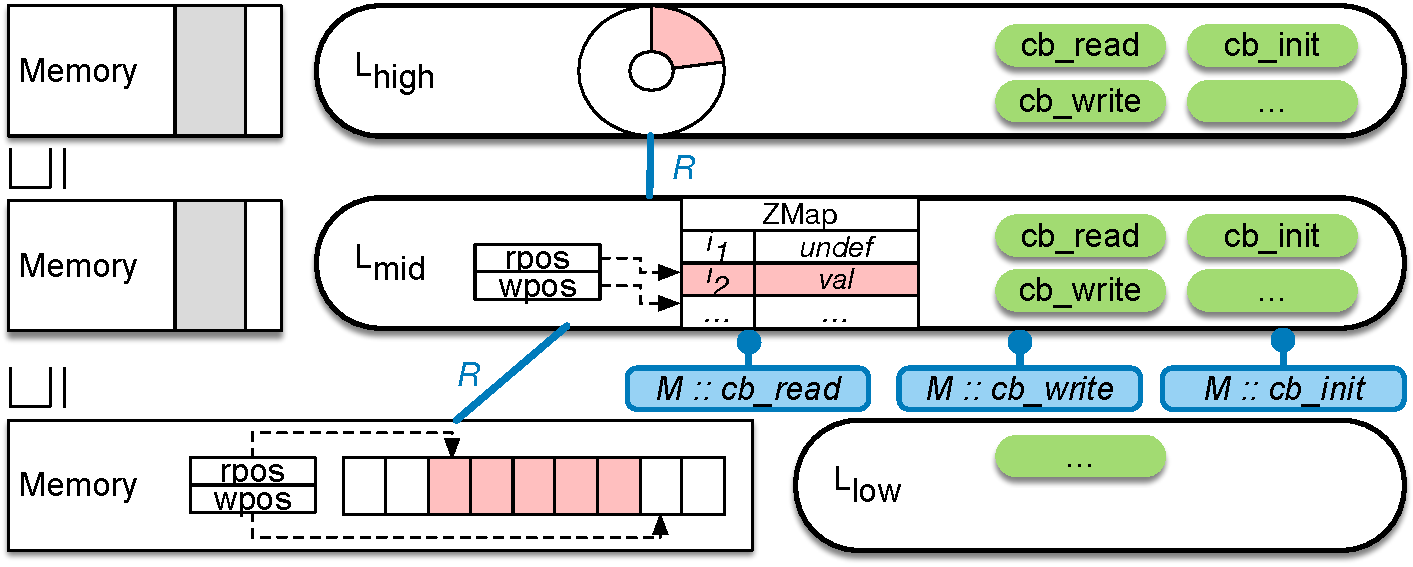
\includegraphics[scale=0.6]{figs/cons_buf}
	\end{center}
	\caption{The layer hierarchy of circular console buffer}
	\label{fig:layer:cons-buf}
\end{figure}

With the support for {\it certified abstraction layers}, we can implement and
specify the circular console buffer, and formally prove the desired property
that the code always satisfies the deep specification in the layer interface.

More formally, let the layer interface defined
in Fig.~\ref{fig:cons_buf_spec} be named $L_{high}$, and the implementation
module in Fig.~\ref{fig:source:cons-buf} be named $M$.
Furthermore, let 
$L_{low}$ define a layer interface when the type of abstract state
is an empty record, and the set of primitives is empty;
$\llbracket{}M\rrbracket{}L$ indicate the behavior of the code module $M$
under the formal semantics of the language $M$ is implemented in (ClightX or LAsm),
instantiated with the layer interface $L$; and $M_1 \oplus M_2$ denote the physical
concatenation of the two individual code modules. Then, the correctness of
the console buffer implementation can be formalized as below:

\begin{lemma}[Correctness of Circular Console Buffer Implementation]
$ $

For every program $P$, there exists a downward simulation from
$\llbracket{}P\rrbracket{}L_{high}$
to $\llbracket{}{P \oplus M}\rrbracket{}L_{low}$.
\end{lemma}

Next, we can define a refinement relation $R$ to relate the concrete circular
buffer in the memory and the abstract list, then prove the contextual refinement
between $\llbracket{}M\rrbracket{}L_{low}$ and $L_{high}$ over the simulation
relation $R$. The forward simulation proof can be achieved on the
primitive-by-primitive basis. One can imagine that due to the non-trivial $R$,
this simulation proof could be complex.

The complexity may further explode when this logical complexity gets mixed with
the complexity of handling the accesses to the CompCert memory. CompCert memory
model is an axiomatized model where the properties are defined through a big
list of axioms without a specific implementation. Any concrete implementation of
this memory model needs to satisfy all the axioms. Thus, one cannot perform any
simple evaluations on the memory, but needs to keep applying appropriate axioms
to derive any desired properties. This severely limits the room for proof
automation and significantly increases the proof size and memory consumption for
proof compilation as the proof gets more complex. To separate the complexity
that comes from the CompCert memory model from the actual complexity of the
proof, in our layered approach, we always make the gap between the underlay and
overlay interface as small as possible when it comes to data abstraction, i.e.,
when a piece of memory gets abstracted into an abstract state at the overlay
interface.

In the case of the circular console buffer, instead of directly jumping from
the in-memory implementation to a logical list, we introduce an intermediate
layer interface where the representation of the circular buffer in the abstract
state is very similar to the one in the memory. We define the intermediate
layer interface $L_{mid}$ with the abstract state $d$ and the primitive specifications
as shown in Fig.~\ref{fig:spec:cons-buf}. Here, for any type $T$, $\mathsf{ZMap}.t~T$
is the type of partial map from integer keys to the values of type $T$.
One can easily observe that the representations shown in Fig.~\ref{fig:spec:cons-buf} are
extremely similar to the actual implementations shown in Fig.~\ref{fig:source:cons-buf}.
Given the similarity, one can easily come up with a refinement relation $R$ which
maps the concrete values in the memory to their appropriate logical values in $d$.
The simulation proof over $R$ is also relatively easy and there is no other
complex factors interfering with the ones from handling the CompCert memory.

Once the contextual refinement between $\llbracket{}M\rrbracket{}L_{low}$ and
$L_{mid}$ is proven, the contextual refinement between $L_{mid}$ and $L_{high}$
can be proven with no code module involved. Thus, this part of proof is completely
logical and the refinement relation $R_{cons\_buf}$ (shown in Fig.~\ref{fig:ref:cons-buf})
in this case only needs to relate two sets of abstract states.
In Fig.~\ref{fig:ref:cons-buf}, \textsf{Abs} is the type of the abstract states
in each layer interface.
The overall layer hierarchy of entire console buffer is shown in Fig.~\ref{fig:layer:cons-buf}.
This kind of two-stage proof strategy
significantly reduces the complexity
of the proof and lifts the main complex proof effort to pure logical level.

\begin{figure}
\[
\begin{array}{lll}
d = ( & \mathsf{cons\_buf\_concrete}: \mathsf{ZMap}.t~\mathbb{Z}, & \vartriangleright \textit{Concrete console buffer} \\
& \mathsf{rpos}: \mathbb{Z}, & \vartriangleright \textit{The head of the buffer} \\
& \mathsf{wpos}: \mathbb{Z}). & \vartriangleright \textit{The tail of the buffer}
\end{array}
\]

\[
\begin{array}{cr}
\inferrule{
	d' = d[\textsf{rpos} \leftarrow 0][\textsf{wpos} \leftarrow 0] \\
}{
	\mathsf{cb\_init} (d) \defeq d'
} & \text{(cb\_init)} \\ [5ex]

\inferrule{
	i = d.\mathsf{rpos} \\
	i \neq d.\mathsf{wpos} \\\\
	c = d.\mathsf{cons\_buf\_concrete}[i] \\
	d' = d[\textsf{rpos} \leftarrow (i + 1)~\textsf{mod}~CB\_SIZE] \\
}{
	\mathsf{cb\_read} (d) \defeq (d', c)
} & \text{(cb\_read\_char)} \\ [3ex]

\inferrule{
	d.\mathsf{wpos} = d.\mathsf{rpos}
}{
	\mathsf{cb\_read} (d) \defeq (d, CB\_EMPTY)
} & \text{(cb\_read\_empty)} \\ [5ex]

\inferrule{
	i = d.\mathsf{wpos} \\
	i' = (i + 1)~\textsf{mod}~CB\_SIZE \\
	d.\mathsf{rpos} \neq i' \\\\
	d' = d[\mathsf{cons\_buf\_concrete}[i \mapsto c]] \\
	d'' = d'[\textsf{wpos} \leftarrow i'] \\
}{
	\mathsf{cb\_write} (d, c) \defeq d'
} & \text{(cb\_write\_char)} \\ [3ex]

\inferrule{
	i = d.\mathsf{wpos} \\
	i' = (i + 1)~\textsf{mod}~CB\_SIZE \\
	d.\mathsf{rpos} = i' \\\\
	i'' = (i' + 1)~\textsf{mod}~CB\_SIZE \\
	d' = d[\mathsf{cons\_buf\_concrete}[i \mapsto c]] \\\\
	d'' = d'[\textsf{wpos} \leftarrow i'][\textsf{rpos} \leftarrow i''] \\
}{
	\mathsf{cb\_write} (d, c) \defeq d''
} & \text{(cb\_write\_overflow)} \\
\end{array}
\]
\caption{Intermediate specifications of console buffer primitives}
\label{fig:spec:cons-buf}
\end{figure}

\begin{figure}
\lstinputlisting [language = Coq] {src/console.v}
\caption{The definition of refinement relation between $L_{high}$ and $L_{mid}$ in Coq}
\label{fig:ref:cons-buf}
\end{figure}

